%\documentclass[aspectratio=169,xcolor=dvipsnames]{beamer}
\documentclass[12pt]{beamer}
\usetheme{AnnArbor}
\setbeamercolor{normal text}{bg=black!10}
\setbeamertemplate{caption}[numbered]
\begin{document}
\title{Hexapod Spider}
\subtitle{Final Project Proposal}
\author[Group 8]{Group 8\\[\baselineskip]Haorong Lu, Xingyuan Wang, Yihua Liu}
\institute{UM-SJTU Joint Institute}
\date{\today}
\begin{frame}
    \titlepage
\end{frame}
\section{Overview}
\begin{frame}{Objectives}
    \begin{itemize}
        \item Implement a hexapod robot with auto collision avoiding.
        \item Control the robot with hand gestures remotely.
    \end{itemize}
\end{frame}

\begin{frame}{Overview}
    \begin{itemize}
        \item Movement with 6 feet and 12 servos.
        \item Implementing stopping, moving forward, moving backward, turning clockwise, and turning counterclockwise.
        \item Controlled through hand gestures using a wearable device with motion tracking device via Bluetooth.
        \item Refusing moving forward when obstacles are detected by ultrasonic distance sensor.
    \end{itemize}
\end{frame}

\section{Mechanical Structure}
\begin{frame}{Mechanical Structure}
    \begin{figure}[H]
        \centering
        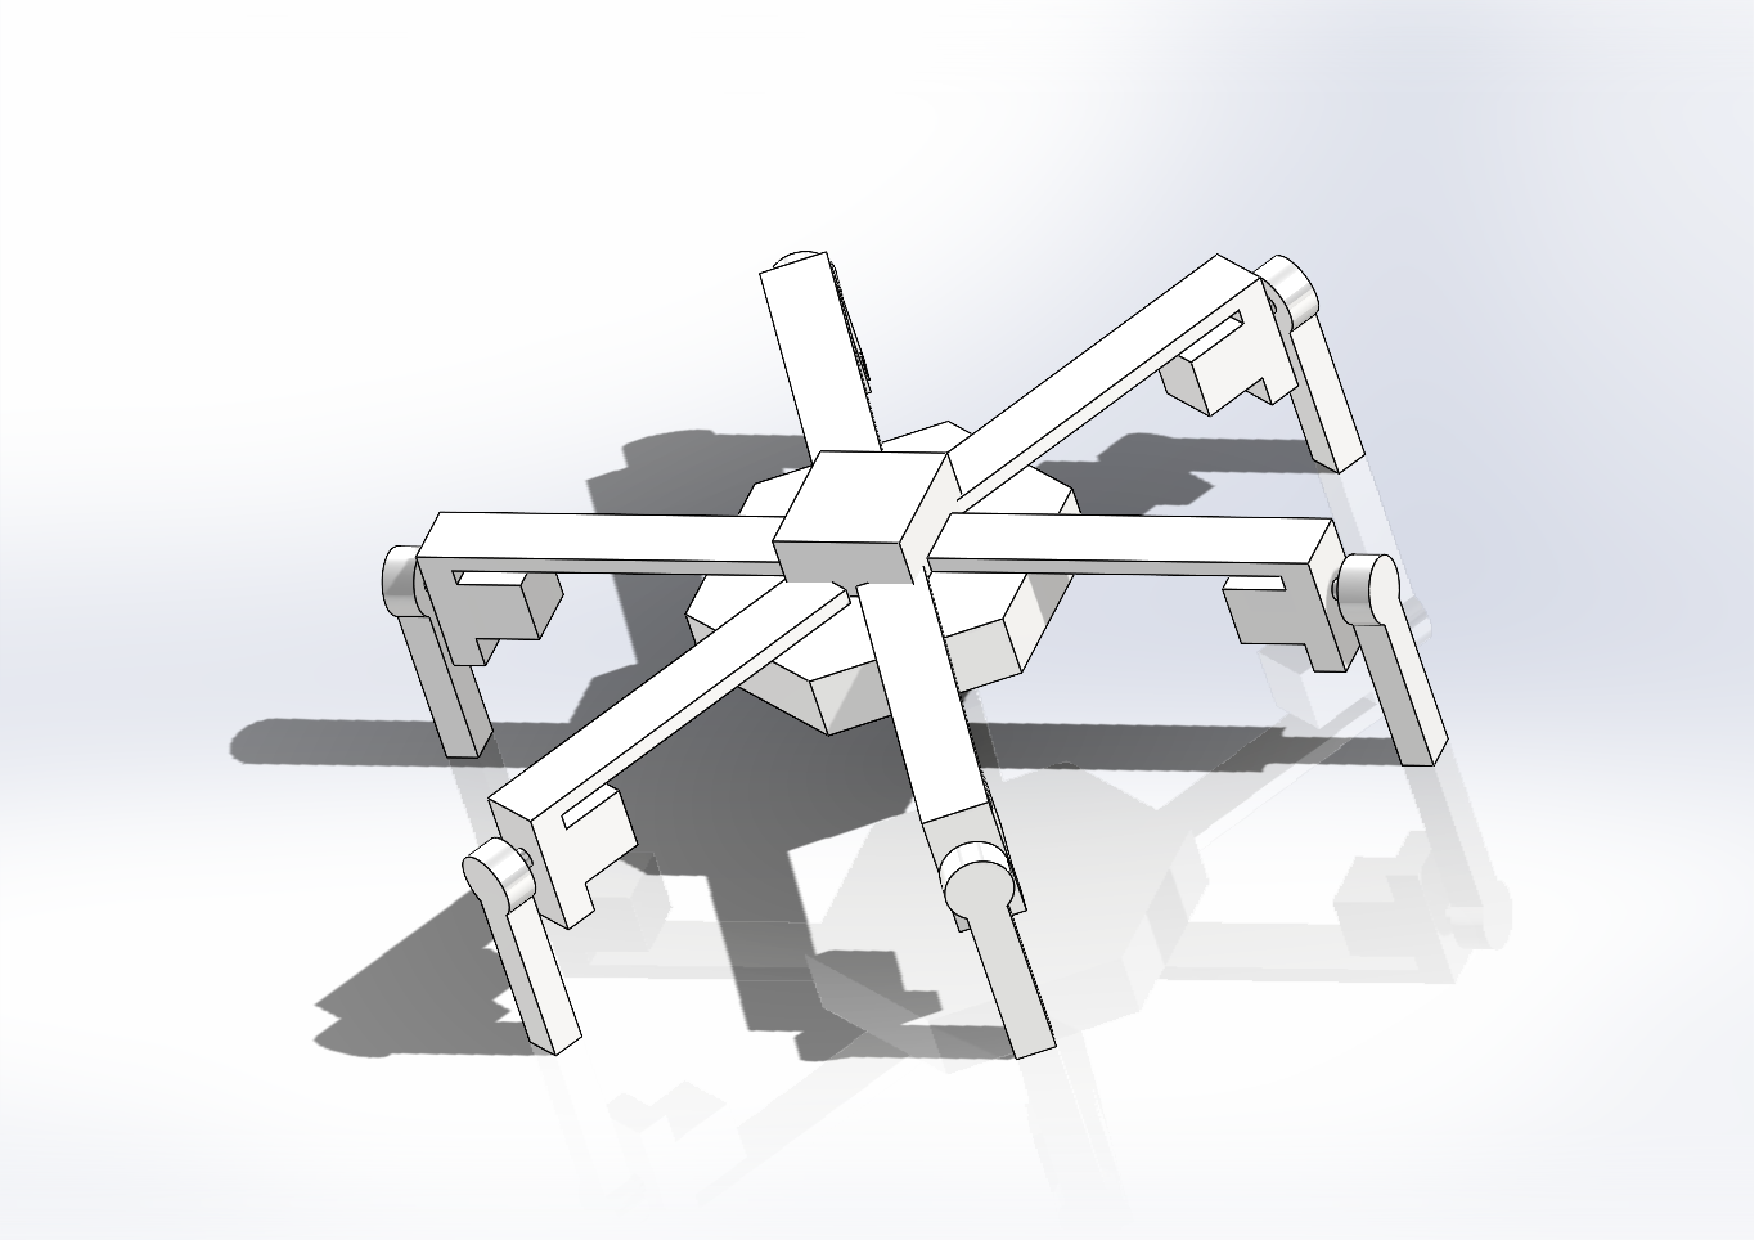
\includegraphics[width=0.75\textwidth]{Mechanical_Structure_2D.pdf}
        \caption{Mechanical Structure.}
    \end{figure}
\end{frame}

\section{Components}
\begin{frame}{Functional Block Diagram}
    \begin{figure}[H]
        \centering
        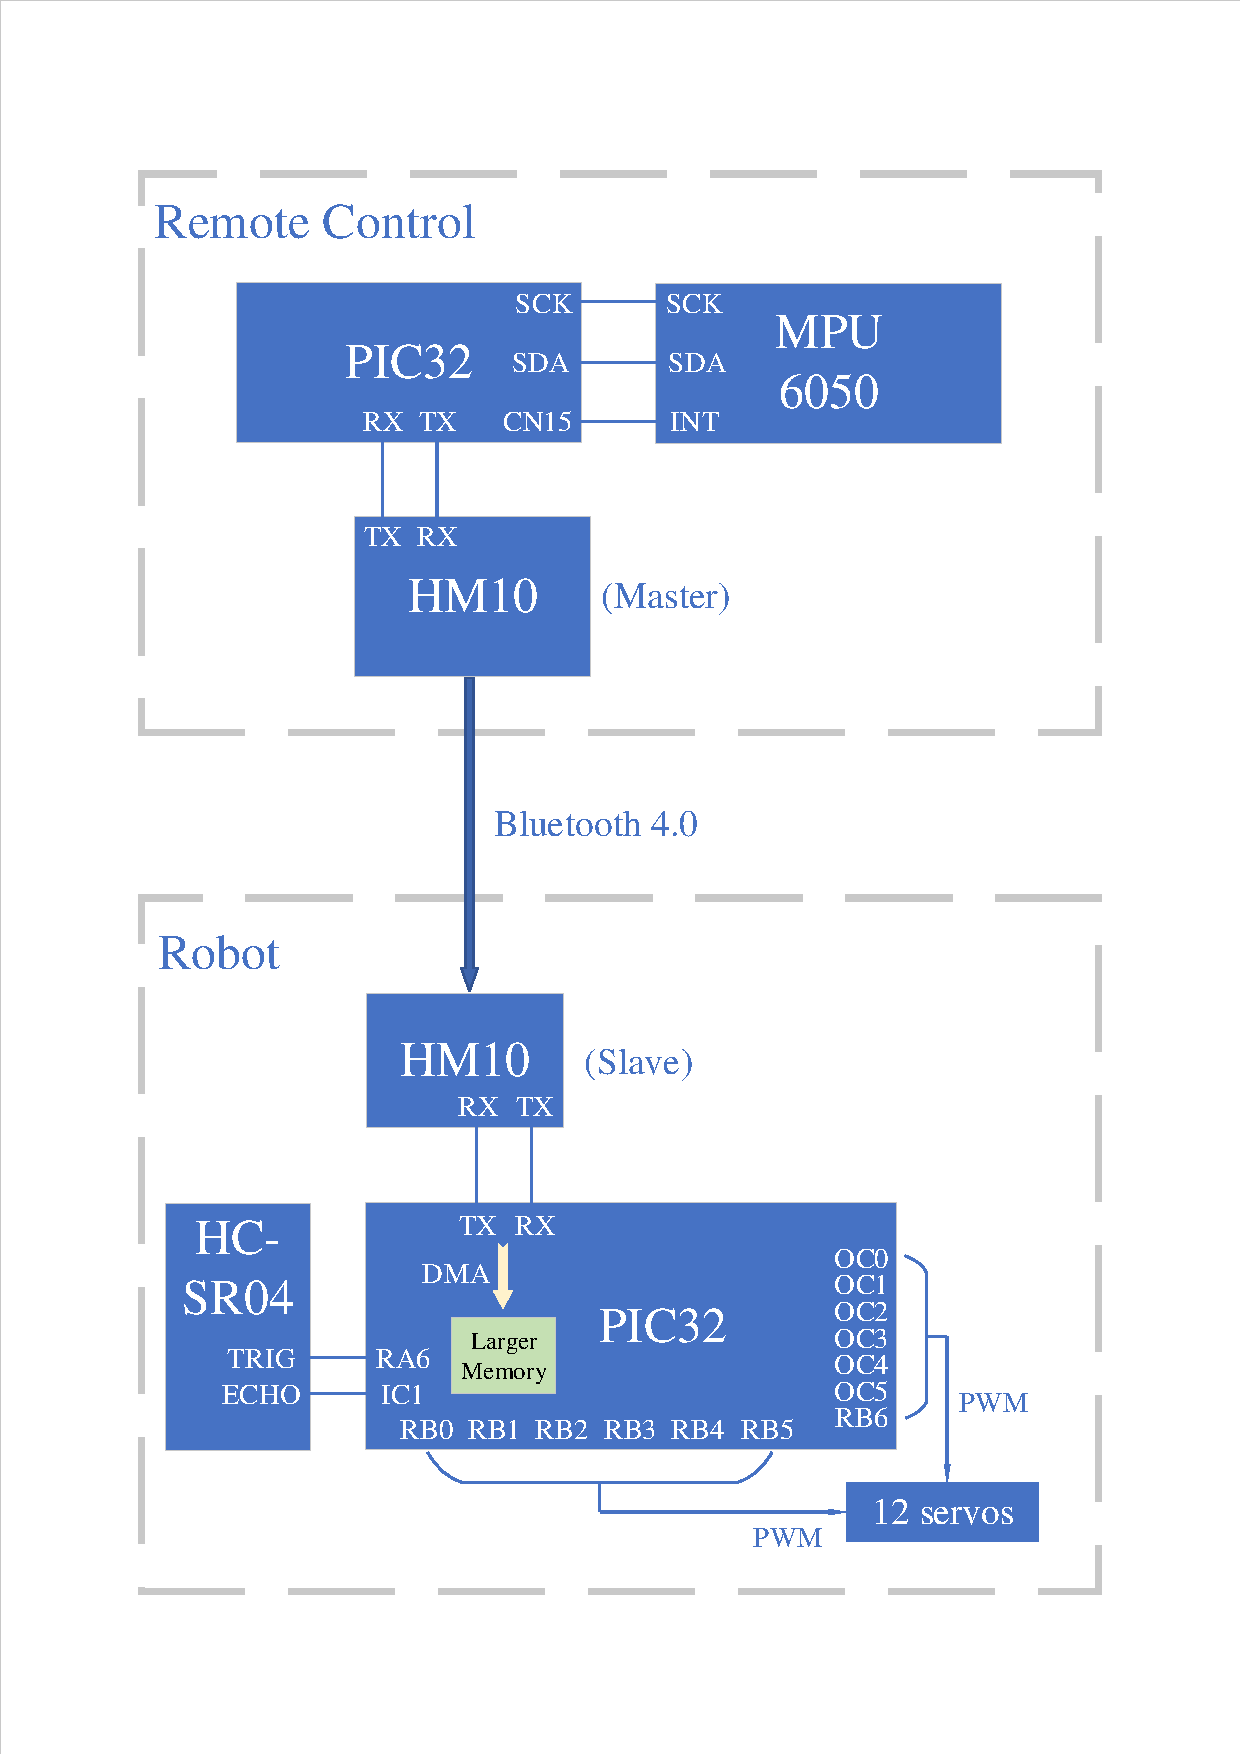
\includegraphics[width=0.45\textwidth]{Diagram.pdf}
        \caption{Functional Block Diagram.}
    \end{figure}
\end{frame}

\begin{frame}{Motion Tracking Device}
    \begin{figure}[H]
        \centering
        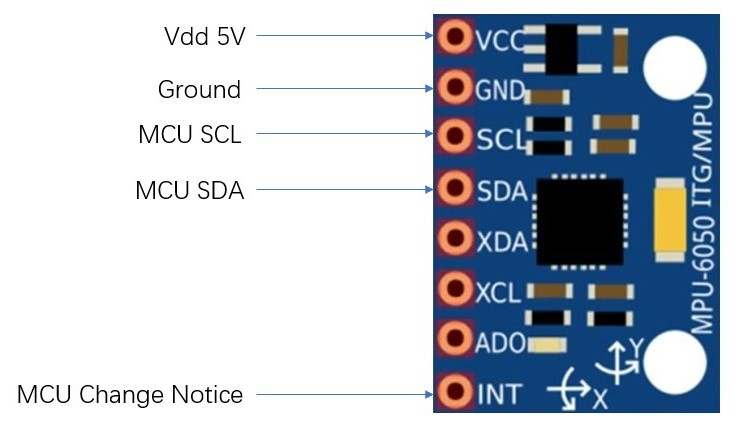
\includegraphics[width=0.5\textwidth]{MPU.jpg}
        \caption{Component diagram of MPU-6050.}
    \end{figure}
    \begin{itemize}
        \item Six DoF (x, y and z axis) accelerometer and gyroscope.
        \item Configuration and data transmission via fast mode I2C.
        \item Programmable internal interrupts and sample rate.
    \end{itemize}
\end{frame}

\begin{frame}{Bluetooth}
    \begin{figure}[H]
        \centering
        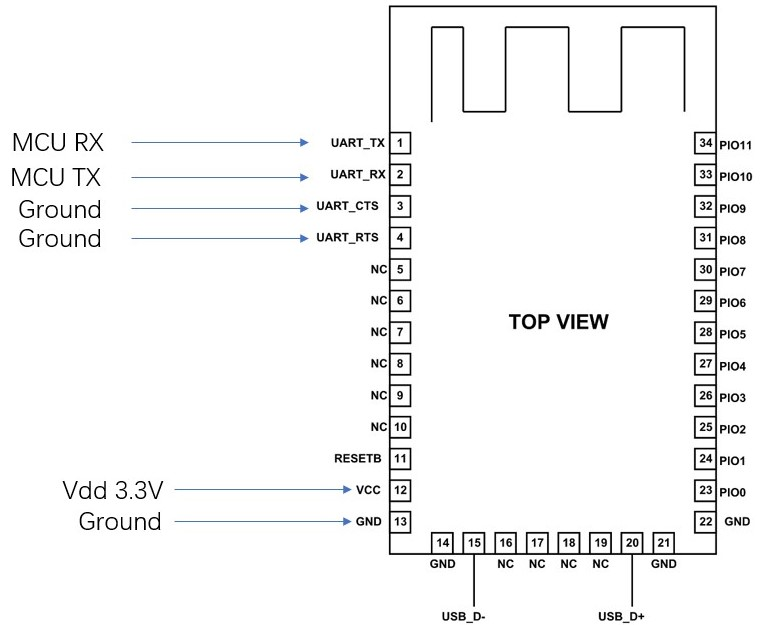
\includegraphics[width=0.4\textwidth]{HM10.jpg}
        \caption{Component diagram of HM-10.}
    \end{figure}
    \begin{itemize}
        \item Communications with MCU via UART at 9600 baud rate.
        \item Programmable master mode and slave mode.
    \end{itemize}
\end{frame}

\begin{frame}{Servo}
    \begin{figure}[H]
        \centering
        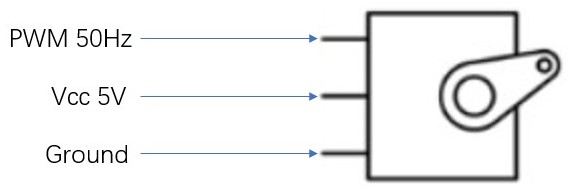
\includegraphics[width=0.6\textwidth]{servo.jpg}
        \caption{Component diagram of MG90S.}
    \end{figure}
    \begin{itemize}
        \item 0-180 degree rotation decided by 50Hz PWM duty cycle.
    \end{itemize}
\end{frame}

\begin{frame}{Distance Detector}
    \begin{figure}[H]
        \centering
        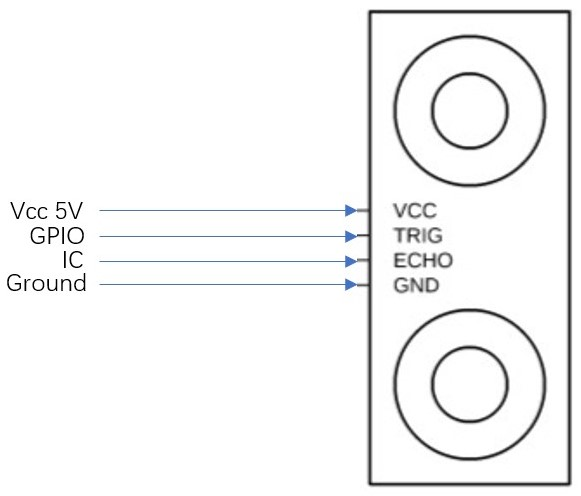
\includegraphics[width=0.4\textwidth]{SR.jpg}
        \caption{Component diagram of HC-SR04.}
    \end{figure}
    \begin{itemize}
        \item Starting ultrasonic wave sending with TRIG pin.
        \item Calculating distance with time of high value in ECHO pin.
    \end{itemize}
\end{frame}

\section{Preliminary Component List}
\begin{frame}{Preliminary Component List}
    \begin{figure}[H]
        \centering
        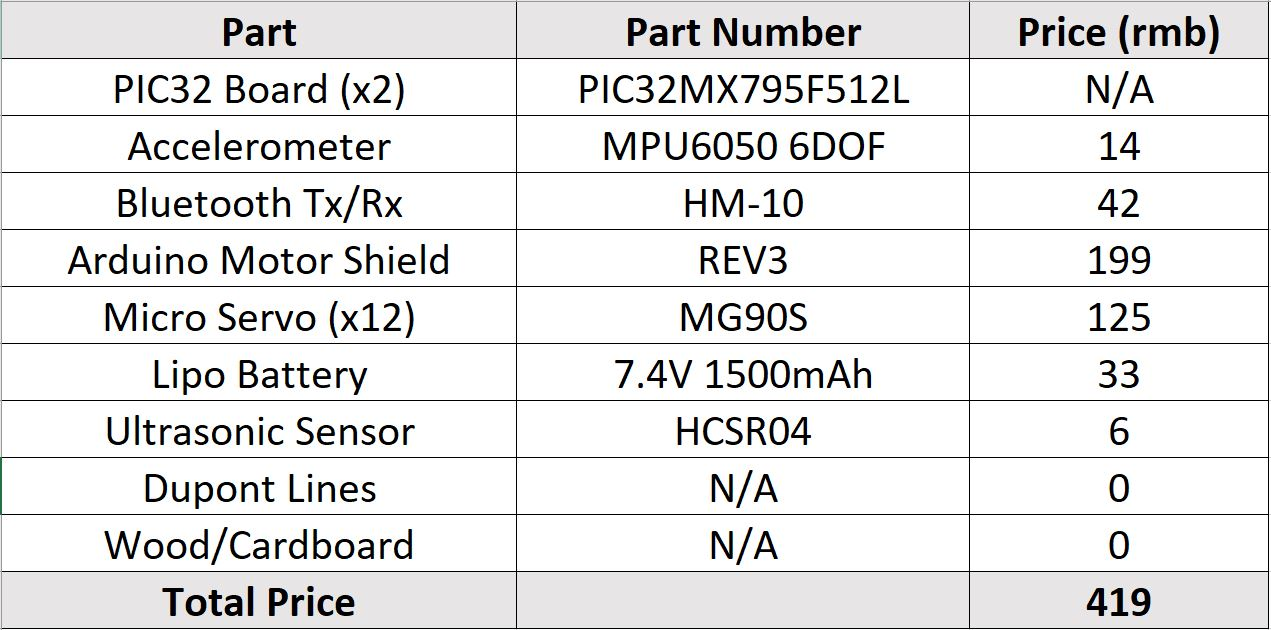
\includegraphics[width=1\textwidth]{materials.JPG}
        \caption{Preliminary Component List for the Hexapod Spider.}
    \end{figure}
\end{frame}

\section{Preliminary Project Timeline}
\begin{frame}{Preliminary Project Timeline}
    \begin{figure}[H]
        \centering
        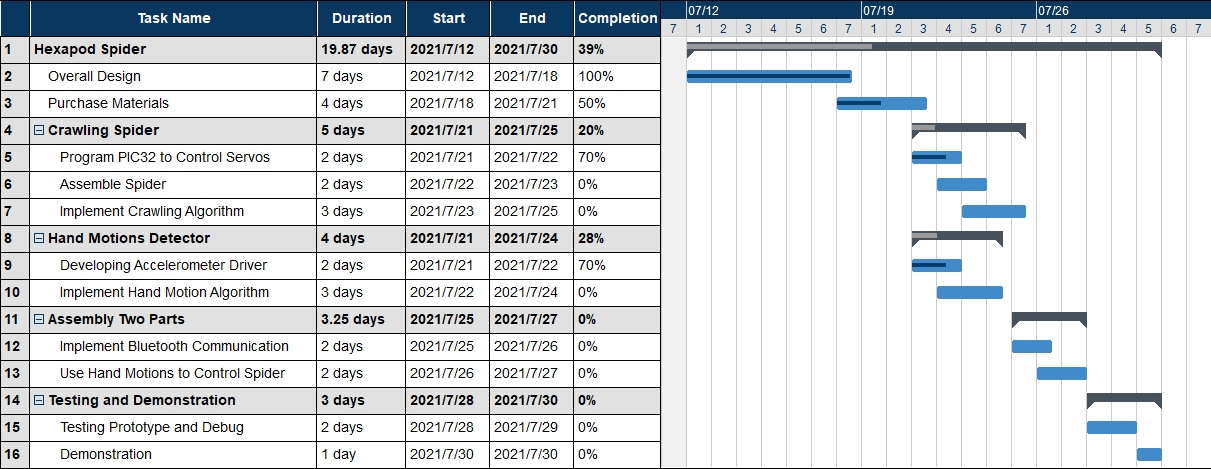
\includegraphics[width=1\textwidth]{Hexapod Spider.jpg}
        \caption{Gantt Chart for developing the Hexapod Spider.}
    \end{figure}
\end{frame}

\section{Q \& A}
\begin{frame}
    \begin{center}
        Q \& A
    \end{center}
\end{frame}

\section{}
\begin{frame}
    \begin{center}
        Thanks!
    \end{center}
\end{frame}

\end{document}